\begin{figure}
\centering
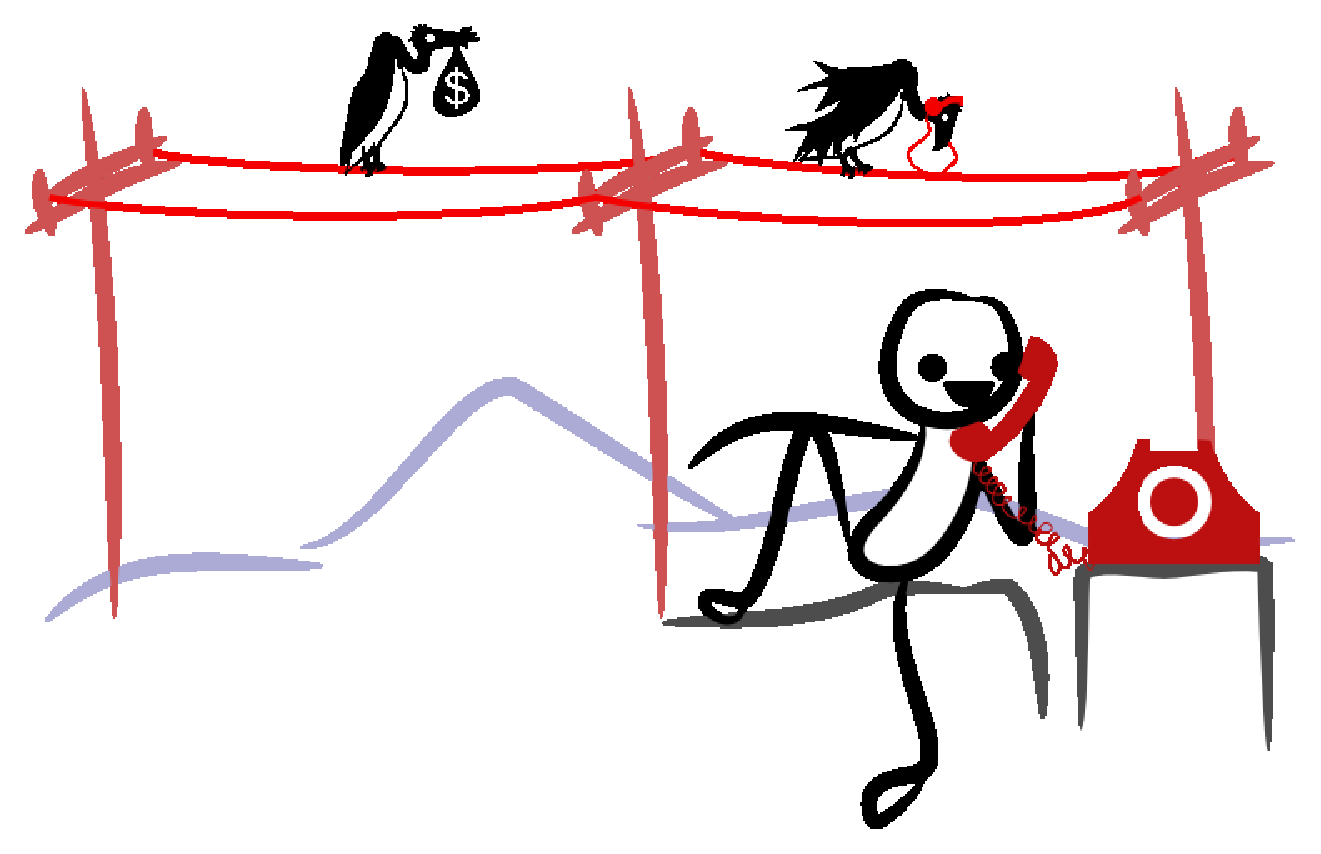
\epsfig{file=assets/buitres.eps, width=0.4\textwidth}
\caption{El gobierno y las empresas se benefician de nuestras telecomunicaciones: tanto monetariamente, como mediante el \textit{surveillance}. El VoIP tiene un costo bajo y provee una comunicación segura, ya que puede ser encriptada. Arte del buitre por Ocal\cite{clker:ocal}}
\end{figure}

\quote{1. La cultura siempre se construye en el pasado.\\
2. El pasado siempre intenta controlar el futuro.\\
3. Nuestro futuro se está volviendo menos libre.\\
4. Para construir sociedades libres, debes limitar el control del pasado.}
\cite{rip:manifesto}

En India al 2014, airtel, la compañía más grande de telecomunicaciones de ese lugar, comenzó a cobrar extra por el servicio de VoIP desde celulares, utilizando servicios como Skype, Viber, Google Hangouts, entre otros, pese a que usar los servicios VoIP es mucho menos costoso que realizar llamadas usando PSTN.\cite{airtel}

En Oman está penado con una multa de 130,317 dólares estadounidenses, y dos años en prisión, realizar llamadas mediante VoIP. En 2009, 212 personas fueron penalizadas por usar VoIP en un café internet.\cite{oman}

En Corea del Sur sólamente se permite usar servicios VoIP autorizados. El costo es muy parecido al de las llamadas mediante PSTN.\cite{korea}

En Estados Unidos, es permitido que las autoridades escuchen conversaciones sobre VoIP sin una orden.\cite{usa}

